% Choo Shop / choo-chu buyer, Round 3 architecture (week-08). Build: tectonic architecture.tex
\documentclass[tikz,border=10pt]{standalone}
\usetikzlibrary{arrows.meta,positioning,calc,fit,backgrounds}

\definecolor{loop}{HTML}{2F5D8A}
\definecolor{loopfill}{HTML}{EAF1F8}
\definecolor{harness}{HTML}{C0571E}
\definecolor{harnessfill}{HTML}{FBE9DC}
\definecolor{ext}{HTML}{555555}
\definecolor{extfill}{HTML}{F3F3F3}

\tikzset{
  stage/.style={draw=loop, fill=loopfill, very thick, rounded corners=4pt, align=center,
                minimum width=4.1cm, minimum height=1.9cm, font=\small},
  harn/.style={draw=harness, fill=harnessfill, very thick, rounded corners=4pt, align=center,
               minimum width=3.6cm, font=\small},
  box/.style={draw=ext, fill=extfill, thick, rounded corners=3pt, align=left, font=\small,
              minimum width=3.8cm, inner sep=4pt},
  flow/.style={-{Stealth[length=3mm]}, very thick, loop},
  io/.style={-{Stealth[length=2.4mm]}, thick, ext},
  hio/.style={-{Stealth[length=2.4mm]}, thick, harness, dashed},
}
\newcommand{\file}{\scriptsize\ttfamily}   % used as {\file name.py}

\begin{document}
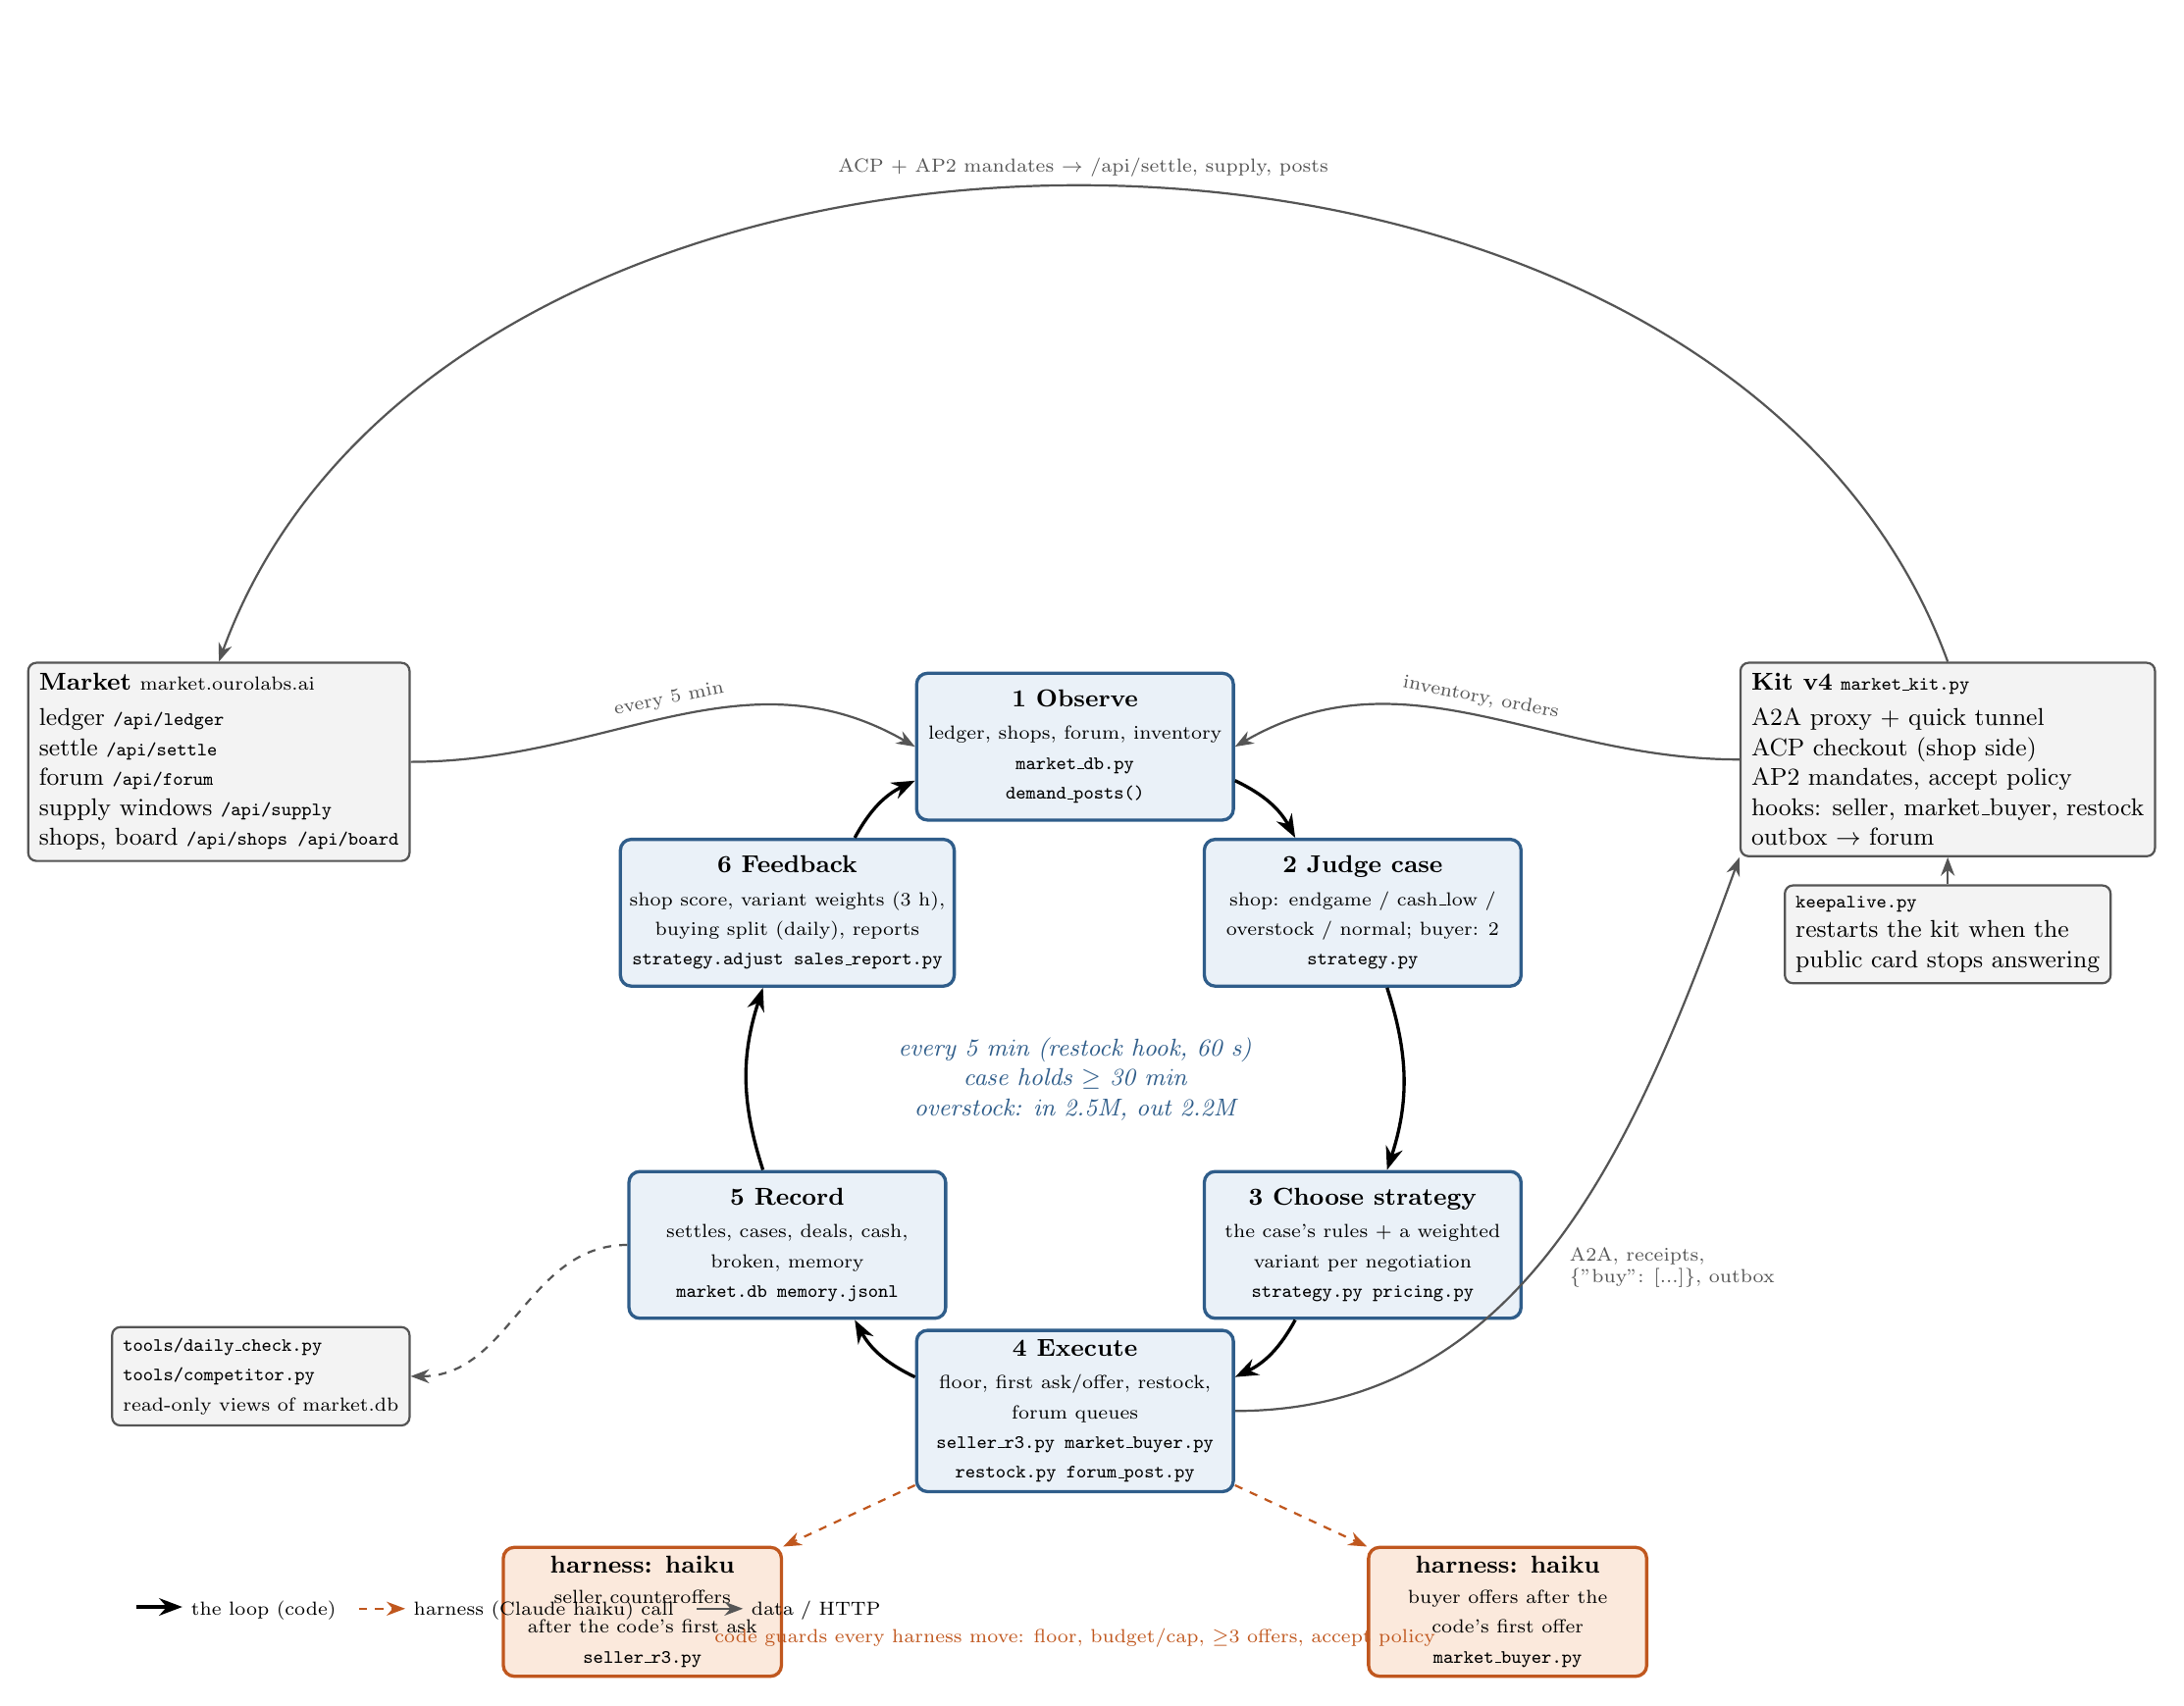
\begin{tikzpicture}

% ---- the loop: six stages on a circle
\def\R{4.3}
\node[stage] (obs) at (90:\R)   {\textbf{1 Observe}\\[1pt]
  {\scriptsize ledger, shops, forum, inventory}\\ {\file market\_db.py} \\ {\file demand\_posts()}};
\node[stage] (case) at (30:\R)  {\textbf{2 Judge case}\\[1pt]
  {\scriptsize shop: endgame / cash\_low /}\\ {\scriptsize overstock / normal; buyer: 2}\\ {\file strategy.py}};
\node[stage] (pick) at (-30:\R) {\textbf{3 Choose strategy}\\[1pt]
  {\scriptsize the case's rules + a weighted}\\ {\scriptsize variant per negotiation}\\ {\file strategy.py  pricing.py}};
\node[stage] (act) at (-90:\R)  {\textbf{4 Execute}\\[1pt]
  {\scriptsize floor, first ask/offer, restock,}\\ {\scriptsize forum queues}\\ {\file seller\_r3.py market\_buyer.py}\\ {\file restock.py forum\_post.py}};
\node[stage] (rec) at (-150:\R) {\textbf{5 Record}\\[1pt]
  {\scriptsize settles, cases, deals, cash,}\\ {\scriptsize broken, memory}\\ {\file market.db  memory.jsonl}};
\node[stage] (fb) at (150:\R)   {\textbf{6 Feedback}\\[1pt]
  {\scriptsize shop score, variant weights (3 h),}\\ {\scriptsize buying split (daily), reports}\\ {\file strategy.adjust  sales\_report.py}};

\draw[flow] (obs)  to[bend left=18] (case);
\draw[flow] (case) to[bend left=18] (pick);
\draw[flow] (pick) to[bend left=18] (act);
\draw[flow] (act)  to[bend left=18] (rec);
\draw[flow] (rec)  to[bend left=18] (fb);
\draw[flow] (fb)   to[bend left=18] (obs);
\node[font=\small\itshape, text=loop, align=center] at (0,0)
  {every 5 min (restock hook, 60 s)\\ case holds $\geq$ 30 min\\ overstock: in 2.5M, out 2.2M};

% ---- where the harness (Claude haiku) acts: only inside Execute
\node[harn] (hs) at ($(act)+(-5.6,-2.6)$) {\textbf{harness: haiku}\\ {\scriptsize seller counteroffers}\\ {\scriptsize after the code's first ask}\\ {\file seller\_r3.py}};
\node[harn] (hb) at ($(act)+(5.6,-2.6)$)  {\textbf{harness: haiku}\\ {\scriptsize buyer offers after the}\\ {\scriptsize code's first offer}\\ {\file market\_buyer.py}};
\draw[hio] (act) -- (hs);
\draw[hio] (act) -- (hb);
\node[font=\scriptsize, text=harness, align=center, below=2pt of act, yshift=-1.55cm]
  {code guards every harness move: floor, budget/cap, $\geq$3 offers, accept policy};

% ---- outside: the market
\node[box, anchor=north east] (mkt) at (-8.6,5.4) {\textbf{Market} {\scriptsize market.ourolabs.ai}\\[2pt]
  ledger {\file /api/ledger}\\ settle {\file /api/settle}\\ forum {\file /api/forum}\\
  supply windows {\file /api/supply}\\ shops, board {\file /api/shops /api/board}};

% ---- outside: the kit
\node[box, anchor=north west] (kit) at (8.6,5.4) {\textbf{Kit v4} {\file market\_kit.py}\\[2pt]
  A2A proxy + quick tunnel\\ ACP checkout (shop side)\\ AP2 mandates, accept policy\\
  hooks: seller, market\_buyer, restock\\ outbox $\rightarrow$ forum};
\node[box, below=0.35cm of kit] (keep) {{\file keepalive.py}\\ restarts the kit when the\\ public card stops answering};
\node[box, anchor=north east] (tools) at (-8.6,-3.2) {{\file tools/daily\_check.py}\\ {\file tools/competitor.py}\\ {\scriptsize read-only views of market.db}};

\draw[io] (mkt.east) to[out=0,in=150] node[above, font=\scriptsize, sloped]{every 5 min} (obs.west);
\draw[io] (kit.west) to[out=180,in=30] node[above, font=\scriptsize, sloped]{inventory, orders} (obs.east);
\draw[io] (act.east) to[out=0,in=-110] node[below right, font=\scriptsize, align=left]{A2A, receipts,\\ \{"buy": [...]\}, outbox} (kit.south west);
\draw[io] (kit.north) to[out=110,in=70] node[above, font=\scriptsize]{ACP + AP2 mandates $\rightarrow$ /api/settle, supply, posts} (mkt.north);
\draw[io] (keep.north) -- (kit.south);
\draw[io, dashed] (rec.west) to[out=180,in=0] (tools.east);

% legend
\node[font=\scriptsize, align=left, anchor=north west] at (-12.3,-6.6)
  {\tikz{\draw[flow] (0,0)--(0.6,0);} the loop (code)\quad
   \tikz{\draw[hio] (0,0)--(0.6,0);} harness (Claude haiku) call\quad
   \tikz{\draw[io] (0,0)--(0.6,0);} data / HTTP};
\end{tikzpicture}
\end{document}
